\documentclass[11pt]{article}
\usepackage[margin=1in]{geometry}
\usepackage[T1]{fontenc}
\usepackage{amsmath,amssymb,bm,booktabs,array,enumitem,xcolor,titlesec,fancyhdr}
\usepackage[most]{tcolorbox}
\usepackage{tikz}
\usetikzlibrary{arrows.meta,positioning,calc}
\usepackage[hidelinks]{hyperref}
\setlength{\parindent}{0pt}\setlength{\parskip}{7pt}
\setlist{itemsep=2pt,topsep=3pt}
\definecolor{blue}{HTML}{000107}\definecolor{card}{HTML}{EFEBF9}\definecolor{cardline}{HTML}{D9D0F0}\definecolor{ink}{HTML}{1F1F2E}\definecolor{red}{HTML}{B5443C}\definecolor{grey}{HTML}{5B5B70}
\titleformat{\section}{\Large\bfseries\sffamily\color{blue}}{\thesection}{0.7em}{}
\titleformat{\subsection}{\large\bfseries\sffamily\color{blue}}{\thesubsection}{0.6em}{}
\titlespacing*{\section}{0pt}{18pt}{6pt}\titlespacing*{\subsection}{0pt}{12pt}{4pt}
\pagestyle{fancy}\fancyhf{}\renewcommand{\headrulewidth}{0pt}
\fancyfoot[C]{\small\color{grey}\thepage}\fancyfoot[L]{\small\color{grey}Project Report}\fancyfoot[R]{\small\color{grey}Tanmay Jain, CERA Lab}
\newtcolorbox{maths}{enhanced,colback=card,colframe=cardline,boxrule=0.6pt,arc=2pt,left=6pt,right=6pt,top=4pt,bottom=4pt,title={\sffamily\bfseries Mathematical formulation},coltitle=blue,colbacktitle=card,attach boxed title to top left={yshift=-2mm,xshift=4mm},boxed title style={colframe=cardline,boxrule=0.6pt,arc=2pt}}
\newtcolorbox{example}{enhanced,colback=white,colframe=cardline,boxrule=0.6pt,arc=2pt,left=6pt,right=6pt,top=4pt,bottom=4pt,title={\sffamily\bfseries Worked example},coltitle=blue,colbacktitle=white,attach boxed title to top left={yshift=-2mm,xshift=4mm},boxed title style={colframe=cardline,boxrule=0.6pt,arc=2pt}}
\newtcolorbox{askbox}{enhanced,colback=white,colframe=blue,boxrule=0.8pt,arc=2pt,left=6pt,right=6pt,top=4pt,bottom=4pt}
\newcommand{\one}{\mathbb{1}}
\newcommand{\bce}{\operatorname{bce}}
\newcommand{\pk}{\mathrm{pk}}
\newcommand{\dep}{\mathrm{dep}}

\begin{document}

{\sffamily\color{blue}\LARGE\bfseries Project Report}\\[2pt]
{\sffamily\large From the simulator, to the fast model that learns from it, to how we score it}\\[4pt]
{\small\color{grey} Tanmay Jain, CERA Lab; results are from previous week (Updated in the weekly update).}

\vspace{4pt}
\begin{askbox}
\textbf{What this document is for.} It walks through the whole project in the order things happen, in plain language, with the mathematics written out where it matters. It defines the variables (each where it first appears, and all together in Section~\ref{sec:symbols}), states the simulator's and the fast model's prediction tasks as known inputs and unknown outputs (Sections~\ref{sub:simproblem} and \ref{sub:learnproblem}), gives the governing equation of each step (the two longest within-system rules are described in words with their thresholds and point to their source files), specifies the evaluation metrics (Section~\ref{sec:score}), and ends with the results to date (Section~\ref{sec:results}). Throughout, three kinds of statement are kept apart: what the simulator \emph{assumes}, what the code \emph{implements}, and what the experiments \emph{showed}.
\end{askbox}

\section*{Overview}

The question the project answers is: \emph{if a coastal storm floods part of New York City, which pieces of infrastructure fail, when, and how many?} The flood itself only knocks out the sites that get wet. Further failures then arise through dependencies: a flooded substation takes down cell towers hours later, a failed pumping station backs up the water network, a hospital on generator power runs out of fuel after four days. That spreading is the \emph{cascade}. In the storms simulated so far it is the larger part of the damage: by 96 hours the total number of failed sites is two to four times the number of directly flooded ones, so more than half of the failures are cascade failures (Section~\ref{sec:results}).

Two tools do the work:

\begin{itemize}
\item \textbf{The simulator} is a rule-based program. Give it a flood map and it plays the cascade forward on a coarse time grid, on a network of 6,231 sites. Because some rules involve chance (which flooded site actually fails, how long a backup lasts), it is run 1,000 times per storm and the results are averaged. One run takes 0.2 to 1.5 seconds; 1,000 runs take up to half an hour.
\item \textbf{The fast model} is a neural network that learns to imitate the simulator. Given the set of sites the flood knocked out directly in one run, plus timing and storm-summary inputs where the model uses them, it returns, for every other site, the probability of having failed by 6, 24, 48 and 96 hours, in 11 milliseconds per run. It is trained on the simulator's runs. Its purpose is to make it possible to scan thousands of storms, which the simulator cannot do in reasonable time (Section~\ref{sub:stormlevel} says how a storm-level answer is assembled from per-run answers).
\end{itemize}

\begin{center}
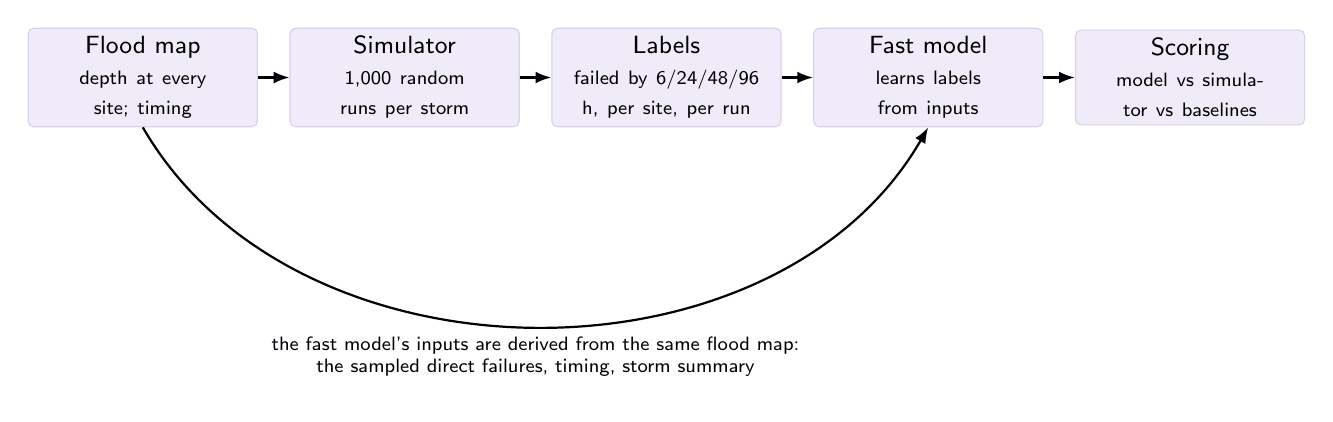
\begin{tikzpicture}[node distance=5mm and 4mm, every node/.style={font=\small\sffamily},
 box/.style={draw=cardline, fill=card, rounded corners=2pt, text width=27mm, align=center, minimum height=11mm, inner sep=3pt},
 arr/.style={-{Latex[length=2mm]}, thick, color=blue}]
\node[box] (flood) {Flood map\\ \scriptsize depth at every site; timing};
\node[box, right=of flood] (sim) {Simulator\\ \scriptsize 1,000 random runs per storm};
\node[box, right=of sim] (lab) {Labels\\ \scriptsize failed by 6/24/48/96 h, per site, per run};
\node[box, right=of lab] (gnn) {Fast model\\ \scriptsize learns labels from inputs};
\node[box, right=of gnn] (score) {Scoring\\ \scriptsize model vs simulator vs baselines};
\draw[arr] (flood) -- (sim); \draw[arr] (sim) -- (lab); \draw[arr] (lab) -- (gnn); \draw[arr] (gnn) -- (score);
\draw[arr] (flood.south) to[out=-60,in=-120] node[below,midway,font=\scriptsize\sffamily,align=center,text width=0.6\textwidth]{the fast model's inputs are derived from the same flood map:\\ the sampled direct failures, timing, storm summary} (gnn.south);
\end{tikzpicture}
\end{center}

The rest of this document follows that arrow from left to right. Section~\ref{sec:network} describes the network. Section~\ref{sec:storm} describes a storm. Sections~\ref{sec:run} and \ref{sec:runs} describe one simulator run and what 1,000 runs give. Section~\ref{sec:model} describes what the fast model is given and what it must return, Section~\ref{sec:compute} how it computes and learns, Section~\ref{sec:score} how we evaluate it, and Section~\ref{sec:results} what the experiments have shown so far.

%======================================================================
\section{The city as a network}\label{sec:network}

\textbf{Sites.} The city is represented by $N = 6{,}231$ sites, each belonging to one of six systems: 203 power substations, 4,150 cell-tower clusters, 61 hospitals, 493 subway stations, 137 water facilities (pumping stations and treatment plants) and 1,187 fuel sites (terminals and gas stations). We write $V$ for the set of all sites, $i$ or $j$ for one site, $a(i)$ for its system, and $V_a$ for all sites of system $a$ (so $N_{\text{telecom}} = 4{,}150$). Each site has a short list of fixed attributes $\mathbf x_i$ (position and a few system-specific facts such as number of towers or bed count), 8 numbers scaled to the range 0--1.

\textbf{Dependency links.} The cascade travels along \emph{dependency links}. A link $(j,i)$ means ``site $i$ needs site $j$ to keep working''. There are 7,513 such links of four kinds: power supply (a substation feeds towers, stations, hospitals, pumps, fuel sites), fuel supply (a terminal or station supplies generators at hospitals, towers and pumps), water supply (a plant supplies a hospital) and SCADA monitoring (a cell cluster carries the control signal of a substation). Each link carries an engineering estimate $\bar b_{ji}$ of how many hours $i$ can keep going after $j$ fails: the \emph{buffer}.

\begin{center}\small
\begin{tabular}{llr}
\toprule
link & what it represents & median buffer $\bar b_{ji}$ (h)\\
\midrule
power $\to$ subway & station loses power & 0 \\
power $\to$ fuel & pump at a gas station or terminal loses power & 0 or 4 \\
power $\to$ water & pumping station on backup & 3 \\
power $\to$ telecom & cell site on battery & 6 \\
power $\to$ hospital & hospital on generator & 96 \\
telecom $\to$ power (SCADA) & substation loses remote control & 2 \\
water $\to$ hospital & hospital's water storage & 24 \\
fuel $\to$ telecom, fuel $\to$ water & generator fuel reserve & 48 \\
fuel $\to$ hospital & generator fuel reserve & 96 \\
\bottomrule
\end{tabular}
\end{center}

\textbf{Other links.} The network file also holds within-system links (power lines, subway lines, water flow, fuel distribution), repair-access links from subway stations, and 23,646 telecom ``failover'' links between neighbouring cell sites of the same carrier. The simulator uses the subway, water and fuel links inside its within-system rules (Step 4 of Section~\ref{sec:run}) and derives the telecom failover partners from site positions; it does not use the repair-access links at all in these campaigns (they describe logistics, and the model has no repair). The fast model sees all of them: 37,355 directed links in 20 relation types, written $E$.

\begin{maths}
$V$: all sites, $|V|=N=6{,}231$. $a(i)\in\{\text{power, telecom, hospital, subway, water, fuel}\}$: system of site $i$. $V_a$, $N_a$: sites of system $a$ and their number. $\mathbf x_i\in[0,1]^8$: fixed attributes. $E^{\dep}$: dependency links $(j,i)$, ``$i$ needs $j$'', with median buffer $\bar b_{ji}\ge0$ hours. $E$: all links, split by relation type $\rho$ into $E_\rho$, 20 types.
\end{maths}

%======================================================================
\section{A storm: what we know before anything fails}\label{sec:storm}

A storm enters the project as a \emph{flood map} from a flood model (Gwyn's GISSR model for most storms; GeoClaw for three). For storm $s$ it gives every site a peak flood depth $d_i^s$ in metres. Sites with $d_i^s>0$ are the \emph{wet sites}, $W^s$. From the storm's hydrograph we also know when the water level peaks, $t^s_{\pk}$ hours after the storm starts, and for every wet site the hour the water arrives, $\alpha_i^s$, how many hours it stays wet, $u_i^s$, and the \emph{lead} $\ell_i^s$: how many hours before the peak the site gets wet. A ``fast'' storm has leads of about 2 hours; a ``slow'' one about 12.

As of October 2026 the project has 70 storms: 22 from earlier work (19 GISSR storms of varied size and 3 GeoClaw maps) and 48 GISSR storms added in October, chosen by a rule written in advance (40 for training, 8 kept unseen). Which of them an experiment trains on is stated with that experiment (Section~\ref{sub:split}).

\begin{maths}
Known for storm $s$: $d_i^s\ge0$ for all $i$; $W^s=\{i:d_i^s>0\}$; $t^s_{\pk}$; and for $i\in W^s$ the hours $\alpha_i^s$, $u_i^s$, $\ell_i^s$ (with $\ell_i^s = t^s_{\pk}-\alpha_i^s$).
\end{maths}

%======================================================================
\section{One simulator run, step by step}\label{sec:run}

\subsection{What the simulator is asked}\label{sub:simproblem}

\begin{askbox}
\textbf{Known.} The dependency links $E^{\dep}$ with their median buffers $\bar b$; the within-system networks and attributes the cascade rules use (subway lines, water-flow and fuel-distribution links, cell-site positions and carriers, hospital beds and health systems), written $E^{\mathrm{sim}}$ together with $E^{\dep}$; the fragility and operational parameters; and, for a storm, the depth map $d^s$ and the timing $(t^s_{\pk},\alpha^s,u^s)$.

\textbf{Unknown.} The failure time of every site, $\mathbf T=(T_i)_{i\in V}$, which is random. What we want is its distribution, summarised as $\pi^s_{ik}=\Pr(\tilde T_i\le t_k\mid s)$ for every site and horizon, where $\tilde T_i$ is the failure time on the label clock (Step 3: hours from 0 for static labels, hours from the peak for arrival labels), and the distribution of the cascade size. There is no formula for these; the simulator estimates them by sampling, as the five steps below describe.
\end{askbox}

\subsection{A run in five steps}

A run is one possible way the storm could play out. The simulator makes two kinds of random draw at the start of a run, then plays the cascade forward deterministically.

\subsubsection*{Step 1. Which sites does the water knock out directly?}

Not every wet site fails. Under the assumed fragility curves, a subway station in 10 cm of water has a high failure probability; a substation in 10 cm of water has a low one. So each wet site fails with a probability that rises with depth, following a \emph{fragility curve} of the standard Hazus form: a lognormal curve with a median depth $\delta_a$ (the depth at which half the sites of that system fail) and a spread $\beta_a$. The simulator then flips a biased coin for each site. The sites that come up ``failed'' are the \emph{seeds} of the run, written $m_i=1$. The 99 sites outside the city footprint never seed.

\begin{maths}
\[
\phi_i^s=\Phi\!\left(\frac{\ln d_i^s-\ln\delta_{a(i)}}{\beta_{a(i)}}\right)\ \text{ if } d_i^s>0 \text{ and } i\in V_{\mathrm{city}},\qquad \phi_i^s=0 \text{ otherwise};
\]
\[
m_i\sim\mathrm{Bernoulli}(\phi_i^s)\ \text{ independently for each site.}
\]
$\Phi$ is the standard normal distribution function (the S-shaped curve from 0 to 1); $V_{\mathrm{city}}$ is the set of 6,132 sites inside the city footprint (the other 99 never seed). Medians $\delta_a$ in metres: power 0.6, telecom 0.3, hospital 0.6, subway 0.1, water 0.5, fuel 0.5. Spreads $\beta_a$: 0.5, 0.6, 0.5, 0.4, 0.5, 0.6. The number of seeds in a run is $n(\mathbf m)=\sum_i m_i$.
\end{maths}

\begin{example}
Three sites, all in 0.3 m of water. Subway station: $(\ln 0.3-\ln 0.1)/0.4 = 2.75$, so $\Phi(2.75)=0.997$: it almost surely fails. Cell cluster: $(\ln 0.3-\ln 0.3)/0.6=0$, so $\Phi(0)=0.5$: a coin flip. Substation: $(\ln 0.3-\ln 0.6)/0.5=-1.39$, so $\Phi(-1.39)=0.08$: it usually survives. At 1 m the substation's probability rises to 0.85.
\end{example}

\subsubsection*{Step 2. How long does each backup last in this run?}

The buffers in the table of Section~\ref{sec:network} are medians. In a real event one hospital's generator runs for three days and another's for six. So in every run each buffer is drawn afresh from a Weibull distribution whose median is the engineering value. The shape of the distribution (how spread out it is) is set per receiving system. Links with a zero buffer stay at zero: a subway station with no power stops immediately.

\begin{maths}
\[
B_{ji}\sim\mathrm{Weibull}(\text{shape }\kappa_{a(i)},\ \text{scale }\lambda_{ji}),\qquad \lambda_{ji}=\frac{\bar b_{ji}}{(\ln 2)^{1/\kappa_{a(i)}}},
\]
which makes the median of $B_{ji}$ exactly $\bar b_{ji}$. Shapes $\kappa$: hospital 2.5, water 2.5, telecom 3.0, power 3.0, fuel 2.0, subway 4.0. Buffers are drawn independently of each other.
\end{maths}

\begin{example}
Power $\to$ hospital, median 96 h, shape 2.5: in 10 \% of runs the generator lasts under 45 h, in 10 \% over 155 h. Power $\to$ telecom, median 6 h, shape 3.0: between 3.2 h and 9.0 h in 80 \% of runs.
\end{example}

\subsubsection*{Step 3. When do the seeds fail? (the two label types)}

The project uses two conventions, and trains a separate fast model for each.

\begin{itemize}
\item \textbf{Static labels.} All seeds fail at the same moment, hour 0, as if the whole flood arrived at once. The cascade is then propagated on the grid $\mathcal G=\{0, 6, 24, 48, 96\}$ hours, with no propagation at hour 0 (hour 0 holds the seeds only).
\item \textbf{Arrival labels} (also called dynamic). Each seed fails at the hour the water actually reaches it, $\alpha_i^s$, kept at its exact value. The cascade is propagated on the grid $\mathcal G^s=\{0,6,12,\dots<t^s_{\pk}\}\cup\{t^s_{\pk}+o:\ o\in\{0,6,24,48,96,144,240,360\}\}$ hours after storm onset. The labels use the storm's peak as their clock: ``failed by 24 h'' means by 24 hours after the peak.
\end{itemize}

Two consequences of the grid are modelling assumptions, not output details: a failure caused by an expired buffer is recorded at the next grid hour, so it can be delayed by up to a grid step relative to continuous time; and under static labels the grid is coarse after 6 h (24, 48, 96). Under arrival labels the cascade gets a head start on sites that flood early. In the 48 storms simulated in October, arrival labels gave 2--50 \% more total failures by 96 h than static labels on the same storm, and above 3.9 m the slow storms ended with about 500 more failed sites than fast storms of the same size (Section~\ref{sec:results}); these are observations from those runs, not consequences that follow from the rules alone.

\subsubsection*{Step 4. How failures spread}

Time moves along the grid. At each grid hour $g$ the simulator applies two rules, over and over, until neither adds a new failure. Failure is permanent: there is no repair in the model. The rules are operational abstractions used in these simulation campaigns, not detailed physical models of each system; their thresholds and where they come from are listed in Section~\ref{sec:assump}.

\textbf{Rule A, dependencies.} A working site fails when one of its suppliers has been failed for longer than the buffer drawn for that link. Every listed dependency is treated as necessary: the loss of any one supplier is enough, and there is no redundancy between suppliers.

\begin{maths}
Let $T_i$ be the hour site $i$ fails ($T_i=\infty$ if it never does). At grid hour $g$:
\[
\text{if } i \text{ is still working and some supplier } j \text{ of } i \text{ has } T_j+B_{ji}\le g,\ \text{ then } T_i\leftarrow g .
\]
\end{maths}

\textbf{Rule B, within a system.} After Rule A, each system checks whether the sites it has lost cause further losses inside the same system:
\begin{itemize}
\item \emph{Subway (overload).} Each station carries a load equal to how many shortest paths pass through it. When stations close, paths reroute and loads shift. A station fails when its new load exceeds its capacity, set at $1.2\times$ its normal load (the Motter--Lai rule). This repeats until no station is over capacity.
\item \emph{Water and fuel (flow).} If a water treatment plant fails, every pumping station upstream of it fails (there is nowhere to send the water). If a fuel terminal fails, every station it supplies fails.
\item \emph{Telecom (capacity and spill).} When a cell site fails, its users move to neighbouring sites of the same carrier within 3 km. With $L^0_i$ the normal demand of site $i$ (its tower count), each site can serve up to a capacity $L^0_i/\rho$, with $\rho=0.6$ its normal busy-hour utilisation; demand it cannot take spills on, for at most two hops. On top of this, demand everywhere is multiplied by a surge $\mu(t)=1+0.5\,e^{-t/12}$, where $t$ is hours since the surge origin (hour 0 for static labels, the peak for arrival labels; $\mu=1$ before it). A site crashes only if the demand offered to it exceeds three times its capacity. Full algorithm: \texttt{src/simulation/intra\_telecom.py}.
\item \emph{Hospital (patient transfer).} Patients of a failed hospital are sent to open hospitals within 40 km, with weights $\propto \text{beds}_k\,e^{-d_{jk}/5\,\text{km}}$, doubled for hospitals in the same health system. A hospital stops accepting at 95 \% of its beds and fails if its census passes 120 \%. Full algorithm: \texttt{src/simulation/intra\_hospital.py}.
\item \emph{Power.} No within-system rule in these campaigns; substations fail by flood or by losing their link (power cascade).
\end{itemize}

Rules A and B feed each other at the same grid hour: a crashed cell cluster can take a substation's SCADA signal (Rule A, 2-hour buffer), the substation's loss can then take further power-dependent sites, and those losses can trigger the within-system rules again.

\subsubsection*{Step 5. What one run gives}

At the end of a run every site has a failure time $T_i$. From it we read, for any hour $t$, whether the site had failed by then. Counting the sites gives the cascade's size at 6, 24, 48 and 96 hours.

%======================================================================
\section{From 1,000 runs to probabilities and labels}\label{sec:runs}

\subsection{Why 1,000 runs}\label{sub:why1000}

One run is one roll of the dice. To say how \emph{likely} a site is to fail, we repeat the run 1,000 times with fresh coin flips and fresh buffers. The failure probability of a site at a horizon is simply the fraction of runs in which it had failed by then. The simulator never outputs a probability directly; probabilities are frequencies over runs.

\begin{maths}
With $R=1{,}000$ runs $r=1,\dots,R$ of storm $s$, horizons $t_1,t_2,t_3,t_4 = 6, 24, 48, 96$ h, and $\tilde T_i^{(r)}$ the failure time of run $r$ on the label clock:
\[
\widehat{\pi}^s_{ik}=\frac1R\sum_{r=1}^{R}\one\!\left[\tilde T_i^{(r)}\le t_k\right]
\]
is the simulator's estimate of the failure probability $\pi^s_{ik}$ of site $i$ by horizon $t_k$. The average cascade size at $t_k$ is $\frac1R\sum_r\sum_i\one[\tilde T_i^{(r)}\le t_k]$.
\end{maths}

\subsection{Labels for the fast model}\label{sub:labels}

Each run becomes one training example. Its label is a table of zeros and ones: for every site and every horizon, did the site fail by then? Static labels count hours from 0; arrival labels count hours from the peak. Because failure is permanent, a row can only go from 0 to 1, never back.

\begin{maths}
\[
\tilde T_i = T_i\ \text{(static)},\quad \tilde T_i = T_i-t^s_{\pk}\ \text{(arrival)};\qquad y_{ik}=\one[\,\tilde T_i\le t_k\,],\qquad y_{i1}\le y_{i2}\le y_{i3}\le y_{i4}.
\]
Hour 0 is not a horizon. Under static labels, hour 0 holds exactly the seed list, which the model is given. Under arrival labels, hour 0 of the label clock is the peak, by which an early-flooding storm already has part of its cascade; the first thing the model is asked for is the state 6 h after the peak.
\end{maths}

\subsection{Which storms train, which storms test}\label{sub:split}

Runs from the \emph{training storms} are shuffled once and split 80/20 into a training set (used to fit the model) and a validation set (used to pick the best epoch and to report numbers). The \emph{held-out storms} are never seen in training; they are the real test of whether the model generalises.

\begin{center}\small
\begin{tabular}{lccc}
\toprule
 & training storms & held-out storms & total\\
\midrule
earlier storms & 17 & 5 & 22\\
new GISSR storms & 40 & 8 & 48\\
all & 57 & 13 & 70\\
\bottomrule
\end{tabular}
\end{center}

With the 17 earlier training storms: 17,000 runs, of which 13,600 train and 3,400 validate; the runs of the 5 held-out storms (5,000) are scored separately, storm by storm. With all 57 training storms: 45,600 train and 11,400 validate (3,400 of them used), scored on the 13 held-out storms; a ``same-effort'' variant trains on the first 13,600 of the 45,600 so that it takes the same number of steps as the 17-storm model.

%======================================================================
\section{The fast model: what it is given, what it must return}\label{sec:model}

\subsection{The learning problem, stated}\label{sub:learnproblem}

The fast model is asked a slightly different question from the simulator. The simulator starts from the depth map and draws the seeds itself. The fast model is handed the seeds of a particular run and asked: \emph{given that exactly these sites were knocked out, how likely is every other site to fail by each horizon?} The only randomness left to average over is the buffers (and, in the within-system rules, nothing: those are deterministic given the failed set).

\begin{askbox}
\textbf{Known (inputs) for one run.} The network $(V,E)$ and attributes $\mathbf X$; the seed indicator $\mathbf m=(m_i)$; and, in the models that use them, the timing inputs $\mathbf Q^s$ and the storm summary $\mathbf c$ (Section~\ref{sub:inputs}). All of these are known before the cascade starts.

\textbf{Unknown (outputs).} For every site and horizon the probability
\[
p^\star_{ik}=\Pr\!\left(Y_{ik}=1\mid \mathbf m,\ s\right),
\]
and from it two derived answers: the expected number of failed sites, $\sum_i p^\star_{ik}$, and each site's most likely failure window.

\textbf{Task.} Find parameters $\theta$ of a network $f_\theta$ such that $f_\theta(\text{inputs})_{ik}\approx p^\star_{ik}$, including on storms the model never trained on.
\end{askbox}

Seeds themselves are not a prediction problem: a seed has $y_{ik}=1$ at every horizon and the model is told which sites are seeds. The training loss still includes them (it averages over all sites, Section~\ref{sub:learn}), which is harmless because the model learns to output 1 for them; every reported metric excludes them and is judged on the \emph{non-seed} sites, $U=\{i:m_i=0\}$.

\subsection{From per-run answers to a storm-level answer}\label{sub:stormlevel}

The simulator's probability $\pi^s_{ik}$ averages over both random draws; the fast model's $p^\star_{ik}$ is conditional on one seed set. The two are linked by averaging the model over seed sets drawn from the fragility probabilities of Step 1, which needs no simulation at all:
\begin{maths}
\[
\Pr(Y_{ik}=1\mid s)=\mathbb E_{\mathbf m\mid s}\big[\Pr(Y_{ik}=1\mid \mathbf m,s)\big]\ \approx\ \frac{1}{R'}\sum_{r=1}^{R'} f_\theta\big(\mathbf m^{(r)},\dots\big)_{ik},
\]
\[
m^{(r)}_i\sim\mathrm{Bernoulli}(\phi_i^s)\ \text{independently for each site and draw.}
\]
\end{maths}
This is what the inference wrapper (\texttt{src/inference/predict\_cascade.py}) does, with $R'=100$ draws by default. So 11 ms is the cost of one conditional prediction; a storm-level estimate with 100 draws costs about a second, against up to half an hour for 1,000 simulator runs. The metrics in Section~\ref{sec:score} score the conditional predictions, run by run, against the simulator's own runs.

\subsection{The input of one site}\label{sub:inputs}

Every site gets one input vector $\mathbf z_i$, assembled from up to four pieces:

\begin{enumerate}
\item \textbf{Fixed attributes} $\mathbf x_i$, 8 numbers (Section~\ref{sec:network}). Current implementation limitation: the elevation and flood-depth slots in the network file hold placeholder constants, so the flood reaches the model only through the next three pieces.
\item \textbf{The storm summary} $\mathbf c$ (added in October 2026; only in the models with the storm-size input). Seven numbers, the same for every site: for each of the six systems, how much of it the flood knocked out directly in this run (that is, the share of seeds), and the same for the city as a whole. Models with timing inputs get three more: the average arrival hour, average hours wet and average lead over the wet sites.
\item \textbf{The seed bit} $m_i$: 1 if the flood knocked out this site.
\item \textbf{Timing} $\mathbf q_i^s$ (only in the models with timing inputs): the site's own arrival hour, hours wet and lead, each divided by 96 hours.
\end{enumerate}

\begin{maths}
\[
c_a=\frac{\ln\big(1+n_a(\mathbf m)\big)}{\ln(1+N_a)}\ \ (a=\text{power},\dots,\text{fuel}),\qquad c_{\mathrm{all}}=\frac{\ln\big(1+n(\mathbf m)\big)}{\ln(1+N)},
\]
and $\bar{\mathbf q}^s$ is the mean of $\mathbf q_i^s$ over the wet sites,
where $n_a(\mathbf m)$ is the number of seeds in system $a$. Each $c$ lies between 0 (no site of that system failed directly) and 1 (all of them did). The logarithm makes the number grow steadily with storm size instead of jumping. If a storm has no wet site with a timing row, $\bar{\mathbf q}^s=\mathbf 0$.
\[
\mathbf q_i^s=\tfrac{1}{96}\,(\alpha_i^s,\ u_i^s,\ \ell_i^s)\ \text{ for wet sites, } \mathbf 0 \text{ otherwise};\qquad
\mathbf z_i=\big[\ \mathbf x_i\ \|\ \mathbf c\ \|\ m_i\ \|\ \mathbf q_i^s\ \big],
\]
with $\|$ meaning ``placed side by side''. Depending on which pieces a model uses, $\mathbf z_i$ has 9, 12, 16 or 22 numbers.
\end{maths}

\begin{example}
Telecom has $N_a=4{,}150$ sites. A run in which the flood knocks out 10 cell clusters directly gives $c_{\text{telecom}}=\ln 11/\ln 4151=0.29$; 100 clusters give $0.55$; 500 give $0.75$. Every site in the city receives these same numbers, so even a tower in the Bronx with no seed near it ``knows'' the storm is large.
\end{example}

Nothing in $\mathbf c$ or $\mathbf q$ comes from the cascade outcome. They are computed from the flood map and the seed list only, so the model is not being shown the answer.

%======================================================================
\section{How the fast model computes and learns}\label{sec:compute}

\subsection{The computation, in four moves}\label{sub:moves}

The model is a graph neural network: it does the same small computation at every site, and lets sites exchange information along links. Its size is 64 numbers per site (the ``hidden state''), two rounds of message passing, four attention heads. All weight matrices $\mathbf W$ and bias vectors $\mathbf b$ below are the trainable parameters $\theta$; there are about 696,000 of them.

\textbf{Move 1: each site summarises its own input.} The input vector is multiplied by a matrix (one per system), a bias is added, and negative entries are set to zero. The result is the site's starting state, 64 numbers.
\begin{maths}
\[
\mathbf h^{(0)}_i=\operatorname{ReLU}\!\left(\mathbf W^{\mathrm{in}}_{a(i)}\mathbf z_i+\mathbf b^{\mathrm{in}}_{a(i)}\right),\qquad \operatorname{ReLU}(x)=\max(x,0).
\]
\end{maths}

\textbf{Move 2: sites aggregate information from their neighbours (twice).} In each round, every site looks at the sites linked to it, separately for each relation type (its power supplier, its fuel supplier, its failover partners, \dots). It does not treat all neighbours equally: it computes an \emph{attention weight} for each neighbour by comparing a ``query'' made from its own state with a ``key'' made from the neighbour's state; the weights are normalised to sum to one. It then takes the weighted sum of the neighbours' ``values'', adds a transformed copy of its own state, sums this over all relation types, adds its previous state (a residual connection: a direct path for the previous hidden state), and applies ReLU. Four attention heads do this in parallel with different matrices and their results are concatenated. After two rounds, every site's state reflects what is within two links of it.

\begin{maths}
For round $l=1,2$, relation $\rho$, head $c$, and $\mathcal N_\rho(i)$ the sites linked to $i$ by relation $\rho$:
\begin{align*}
\alpha^{(l,c)}_{ij,\rho}&=\operatorname*{softmax}_{j\in\mathcal N_\rho(i)}\frac{\big(\mathbf W^{(l,c)}_{Q,\rho}\mathbf h^{(l-1)}_i\big)^{\!\top}\big(\mathbf W^{(l,c)}_{K,\rho}\mathbf h^{(l-1)}_j\big)}{\sqrt{16}}
\qquad\text{(attention weights, sum to 1 over } j\text{)}\\
\mathbf g^{(l)}_{i,\rho}&=\Big\|_{c=1}^{4}\sum_{j\in\mathcal N_\rho(i)}\alpha^{(l,c)}_{ij,\rho}\,\mathbf W^{(l,c)}_{V,\rho}\mathbf h^{(l-1)}_j\ +\ \mathbf W^{(l)}_{S,\rho}\mathbf h^{(l-1)}_i
\qquad\text{(message from relation }\rho\text{)}\\
\mathbf h^{(l)}_i&=\operatorname{ReLU}\!\Big(\sum_{\rho\ \text{ending at } a(i)}\mathbf g^{(l)}_{i,\rho}+\mathbf h^{(l-1)}_i\Big)
\qquad\text{(new state)}
\end{align*}
\end{maths}

\textbf{Why local message passing produced a storm-size bias.} After two rounds, a site's state depends only on inputs within two links of it. Before the storm summary existed, a site with no seed within two links received exactly the same inputs in a small storm and a huge one, so the model had to give it the same answer: an average. That is why the model over-counted a small unseen storm by 3--4 times and under-counted big ones by a third (Section~\ref{sec:results}). Giving every site the storm summary $\mathbf c$ supplies the storm's size to every site while keeping two rounds of local message passing; it does not let a site see distant failure configurations or long dependency paths.

\textbf{Move 3: each site turns its final state into four raw numbers.} A small two-layer network (one per system) maps the 64-number state to 4 numbers $\eta_{i1},\dots,\eta_{i4}$, one per horizon.
\begin{maths}
\[
\bm\eta_i=\mathbf W^{(2)}_{a(i)}\operatorname{ReLU}\!\left(\mathbf W^{(1)}_{a(i)}\mathbf h^{(2)}_i+\mathbf b^{(1)}_{a(i)}\right)+\mathbf b^{(2)}_{a(i)} .
\]
\end{maths}

\textbf{Move 4: raw numbers become probabilities that can only go up.} ``Failed by 48 h'' can never be less likely than ``failed by 24 h''. To guarantee this, the four raw numbers are read as \emph{hazards}: $h_{ik}$ is the chance the site fails \emph{during} window $k$ given it survived the earlier windows. The chance of surviving all windows up to $k$ is the product of $(1-h)$; one minus that is the probability of having failed by $t_k$.
\begin{maths}
\[
h_{ik}=\sigma(\eta_{ik})=\frac{1}{1+e^{-\eta_{ik}}},\qquad S_{ik}=\prod_{j\le k}(1-h_{ij}),\qquad p_{ik}=1-S_{ik}.
\]
\end{maths}

\begin{example}
Raw outputs $\bm\eta_i=(-2,-1,0,1)$. Hazards: $h=(0.12,\ 0.27,\ 0.50,\ 0.73)$. Survival: $S=(0.88,\ 0.64,\ 0.32,\ 0.09)$. Probabilities of having failed by 6, 24, 48, 96 h: $p=(0.12,\ 0.36,\ 0.68,\ 0.91)$. They rise, as they must.
\end{example}

\subsection{How the parameters are learned}\label{sub:learn}

Training means adjusting the 696,000 parameters so that the model's probabilities match the simulator's labels. The yardstick is the \emph{log loss} (binary cross-entropy): for one site and horizon it is $-\ln p$ if the site failed and $-\ln(1-p)$ if it did not. It is small when the model gives high probability to what happened and very large when the model is confidently wrong.

\begin{example}
The site failed ($y=1$). Model says $p=0.9$: loss $-\ln 0.9=0.11$. Model says $p=0.5$: loss $0.69$. Model says $p=0.1$: loss $2.30$. Being sure and wrong costs twenty times more than being sure and right.
\end{example}

The loss of a run is the average over all 6,231 sites (seeds included) and 4 horizons; it is a binary cross-entropy on the cumulative ``failed by $t_k$'' outcomes, and the hazard read-out only guarantees that the four probabilities rise (this is not the likelihood of a discrete-time survival model, which would score the failure window itself). Training goes through the training runs one at a time (13,600 for the 17-storm models): compute the loss, compute how each parameter should move to reduce it (the gradient, by back-propagation), and take a small step in that direction with the Adam optimiser. Six passes over the data are made. After each pass the loss on the 3,400 validation runs is measured, and the version of the model with the lowest validation loss is kept.

\begin{maths}
\[
\bce(p,y)=-\,y\ln p-(1-y)\ln(1-p),\qquad
\mathcal L(\theta;\text{run})=\frac{1}{N\cdot 4}\sum_{i\in V}\sum_{k=1}^{4}\bce\big(p_{ik},y_{ik}\big),
\]
\[
\hat\theta=\arg\min_\theta\ \frac{1}{|\mathcal D_{\mathrm{tr}}|}\sum_{\text{runs}\in\mathcal D_{\mathrm{tr}}}\mathcal L(\theta;\text{run}).
\]
Adam, learning rate $10^{-3}$, weight decay $10^{-5}$, dropout $0.1$, 6 epochs. The initial parameters are random; since October 2026 each setting is trained from two different random starts (PyTorch seeds 1 and 2) so that we can see how much results move between starts.
\end{maths}

\subsection{The baselines: three predictors with no neural network}\label{sub:baselines}

To know whether the model has learned anything worth having, it is compared with three simple predictors built from the same training runs. Each knows a little more than the last.

\begin{enumerate}
\item \textbf{Base rate.} Every non-seed site gets the same number: the overall fraction of non-seed sites that fail by that horizon in the training runs.
\item \textbf{Site frequency.} Each site gets its own failure frequency over all training runs, ignoring which storm it is.
\item \textbf{Lookup table.} For each training storm, record each site's failure frequency in that storm's runs. For a new run, count its seeds, find the training storm with the closest average number of seeds, and reuse that storm's frequencies. This predictor knows the size of the storm and nothing else.
\end{enumerate}

\begin{maths}
With $n_i$ the number of training runs in which site $i$ is not a seed, $\mathcal D^s_{\mathrm{tr}}$ the training runs of storm $s$ and $n^s_i$ defined likewise:
\[
\bar f_k=\frac{\sum_{\text{runs}}\sum_i(1-m_i)\,y_{ik}}{\sum_{\text{runs}}\sum_i(1-m_i)},\qquad
f_{ik}=\frac{\sum_{\text{runs}}(1-m_i)\,y_{ik}+0.5}{n_i+1},
\]
\[
f^{s}_{ik}=\frac{\sum_{\text{runs}\in\mathcal D^s_{\mathrm{tr}}}(1-m_i)\,y_{ik}+f_{ik}}{n^s_i+1}.
\]
The lookup predicts $p_{ik}=f^{s^\star}_{ik}$ with $s^\star$ the training storm whose mean seed count is closest to $n(\mathbf m)$. The small additions ($+0.5$, $+f_{ik}$) keep frequencies away from exactly 0 or 1.
\end{maths}

%======================================================================
\section{How we evaluate and compare models}\label{sec:score}

Every metric is computed on non-seed sites, over the runs being scored: either the 3,400 validation runs or the 1,000 runs of one held-out storm. Log loss, Brier score, AP and AUC are computed per run and then averaged over runs; count bias and count error are ratios of sums over runs; precision, recall, failure-window accuracy and calibration pool the site-run pairs. The same code scores the model and each baseline, so they are always compared on identical runs.

\subsection{Per-site probability error: log loss}\label{sub:bce}

The same quantity as the training loss, but restricted to non-seed sites and reported per horizon and averaged over the four. Lower is better; 0 would be perfect; always answering ``50 \%'' scores $\ln 2 = 0.69$.
\begin{maths}
\[
\mathrm{BCE}_k=\text{mean over runs of }\ \frac{1}{|U|}\sum_{i\in U}\bce(p_{ik},y_{ik}),\qquad \mathrm{BCE}=\tfrac14\sum_{k=1}^4\mathrm{BCE}_k.
\]
The Brier score is the same with $(p-y)^2$ in place of $\bce$.
\end{maths}

\subsection{Does the model get the size of the cascade right? Count bias and count error}\label{sub:count}

The model outputs probabilities, not a count. The count it implies is the \emph{expected} number of failed sites, which is the sum of the probabilities: if 100 sites each have a 30 \% chance, we expect 30 failures. There is no cut-off at 50 \%. The simulated count is the number of non-seed sites that actually failed in the run.

Two numbers are reported. \emph{Bias} asks whether the model is too high or too low on average; it can hide errors that cancel between runs. \emph{Count error} (WAPE) adds up the size of every miss regardless of sign, so it cannot be fooled by cancellation.

\begin{maths}
Per run: $\hat C_k=\sum_{i\in U}p_{ik}$ (predicted), $C_k=\sum_{i\in U}y_{ik}$ (simulated). Over the runs scored (undefined if no non-seed site fails in any of them):
\[
\mathrm{Bias}_k=\frac{\sum_{\text{runs}}\big(\hat C_k-C_k\big)}{\sum_{\text{runs}}C_k},\qquad
\mathrm{WAPE}_k=\frac{\sum_{\text{runs}}\big|\hat C_k-C_k\big|}{\sum_{\text{runs}}C_k}.
\]
``Predicted $\div$ simulated'' on the slides is $1+\mathrm{Bias}_k$ (1.0 is correct). Usually reported at 96 h.
\end{maths}

\begin{example}
Three sites with probabilities 0.8, 0.5 and 0.1 contribute $1.4$ expected failures. A run where the simulator has 200 non-seed failures and the model's probabilities add to 290 has a miss of 90; if every run looked like that, bias and count error would both be $90/200=45\,\%$. If half the runs were $+90$ and half $-90$, bias would be 0 but count error still 45 \%.
\end{example}

\subsection{Does it rank the right sites highest? AP and AUC}\label{sub:rank}

These two ignore the level of the probabilities and look only at their \emph{order}. Sort the non-seed sites from most to least likely to fail. \emph{Average precision} (AP) walks down that list and, each time it reaches a site that really failed, notes what fraction of the sites so far really failed; AP is the average of those fractions, and equals 1 when every failing site is ranked above every surviving one. \emph{AUC} is the probability that a randomly chosen failing site is ranked above a randomly chosen surviving site. A model can have a high AP and still get the count badly wrong, which is exactly what happened before the storm summary.

\begin{maths}
With $P_n$, $R_n$ the precision and recall after the $n$-th distinct score ($R_0=0$), $n_+$ failing and $n_-$ surviving sites, and ranks assigned in ascending order of $p_{ik}$ with average ranks for ties:
\[
\mathrm{AP}=\sum_n (R_n-R_{n-1})\,P_n,\qquad
\mathrm{AUC}=\frac{\sum_{i:\,y_i=1}\operatorname{rank}(i)-n_+(n_++1)/2}{n_+\,n_-}.
\]
Computed per run and horizon, then averaged over the runs in which both classes occur (a run with no failing or no surviving site gives no value and is left out).
\end{maths}

\subsection{Yes/no flags}

If a planner needs a list, sites with $p_{ik}\ge0.5$ are flagged. Precision is the share of flagged sites that fail; recall is the share of failing sites that were flagged. Both are pooled over runs.

\subsection{Does it get the timing right? Failure windows}\label{sub:window}

The four cumulative probabilities define five windows: by 6 h, 6--24 h, 24--48 h, 48--96 h, and ``not by 96 h''. The probability mass in each window is the difference between consecutive cumulative probabilities. The timing metric is conditional on failure: among the non-seed sites that really fail by 96 h, we ask whether the most likely of the four failure windows is the true one, pooling sites over runs. (A five-class version that also scores ``not by 96 h'' is stored alongside, with that window predicted when $p_{i4}<0.5$.)

\begin{maths}
\[
w_{i1}=p_{i1},\quad w_{ij}=p_{ij}-p_{i,j-1}\ (j=2,3,4),\quad w_{i5}=1-p_{i4};\qquad
\text{true window } j^\star_i=5-\sum_k y_{ik};
\]
\[
\mathrm{Acc}_{\mathrm{win}}=\frac{\#\{\text{failing non-seed sites with }\arg\max_{j\le4}w_{ij}=j^\star_i\}}{\#\{\text{failing non-seed sites}\}}.
\]
\end{maths}

\begin{example}
From the earlier example, $p=(0.12,0.36,0.68,0.91)$ gives the window masses $(0.12,0.24,0.32,0.23,0.09)$, so the model's best guess is that the site fails between 24 and 48 hours.
\end{example}

\subsection{Are the predicted probabilities calibrated?}\label{sub:ece}

Take all the site-run pairs where the model said ``about 30 \%''. If about 30 \% of them really failed, the model is calibrated. The expected calibration error (ECE) sorts the pairs into ten probability bins and averages the gap between the stated probability and the observed failure rate.
\begin{maths}
\[
\mathrm{ECE}_k=\sum_{b=1}^{10}\frac{|\mathcal B_b|}{n}\,\Big|\,\overline{p}_{b}-\overline{y}_{b}\,\Big| ,\qquad \overline{p}_b=\frac{1}{|\mathcal B_b|}\sum_{(i,\text{run})\in\mathcal B_b}p_{ik},\quad \overline{y}_b=\frac{1}{|\mathcal B_b|}\sum_{(i,\text{run})\in\mathcal B_b}y_{ik},
\]
$n$ being the number of site-run pairs and $\mathcal B_b$ the pairs whose $p_{ik}$ falls in bin $b$: the bin-size-weighted gap between stated probability and observed failure rate.
\end{maths}

\subsection{Speed}

Wall time of one forward pass of the model (all 6,231 sites, four horizons; one run at a time; inputs already on the device; median of 50 timed passes after 5 warm-up passes on an NVIDIA L40S) against the wall time of one simulator run on a CPU core: 11 milliseconds against 0.2--1.5 seconds. Building the inputs and moving them to the GPU is not included.

\subsection{How comparisons are decided}

\begin{itemize}
\item The model \emph{beats} a baseline on a set of runs if its log loss is lower there.
\item With two random starts per setting, an improvement is called \emph{consistent across the tested initialisations} only if both runs of one setting beat both runs of the other. This is a transparency rule, not a significance test.
\item Validation runs come from the training storms, so a model can do well there by recognising the storm. Generalisation is judged on held-out storms only.
\item Every experiment's pass/fail thresholds are written into the scoring script before the run (for example: ``validation count error at 96 h must fall to 0.30 or below''). The script prints PASS or MISS; misses are reported as such.
\end{itemize}

%======================================================================
\section{Results to date}\label{sec:results}

Each result below is dated and names the runs it comes from. Full tables are in the repository (\texttt{analysis/gnn/}).

\subsection{What the simulator produced (label campaign of 7 October 2026)}

The 48 storms added in October were each simulated 1,000 times under both label conventions (96 of 96 runs complete; an identity check reproduced an earlier campaign's record exactly).
\begin{itemize}
\item \textbf{Cascade against direct damage.} Under static labels the total number of failed sites by 96 h was 2 to 4 times the number of directly flooded sites, depending on the storm (for example 133 failed sites from 60 flooded at a 1.9 m peak; 2,660 from 660 at 4.7 m).
\item \textbf{Arrival against static labels.} Arrival labels gave 2--50 \% more total failures by 96 h than static labels on the same storm, with a step near a 3.2 m peak (about 2,300 to 3,000 sites).
\item \textbf{Slow against fast storms.} Above a 3.9 m peak, storms whose sites were wet about 12 h before the peak ended with 3,630--3,720 failed sites; storms with 2--2.6 h leads ended with 3,090--3,190 (one exception at 4.23 m), and varied about three times as much from run to run.
\end{itemize}

\subsection{The fast model before and after the storm summary (7 October 2026)}

Setting: the 17 earlier training storms, four models (static or arrival labels $\times$ mask-only or timing inputs), each trained from two random starts with and without the storm summary. Six pass/fail criteria were written into the scoring script before training; all six passed. Values in the table are means of the two starts; ``lookup'' is the nearest-storm table of Section~\ref{sub:baselines}.

\begin{table}[t]\centering\small
\setlength{\tabcolsep}{4pt}
\begin{tabular}{@{}p{0.36\textwidth}cccc@{}}
\toprule
validation (3,400 runs of the training storms) & static, mask & static, +timing & arrival, mask & arrival, +timing\\
\midrule
log loss, without $\to$ with summary & $0.081\to0.045$ & $0.073\to0.045$ & $0.162\to0.071$ & $0.140\to0.069$\\
log loss, lookup & 0.071 & 0.071 & 0.095 & 0.095\\
count error at 96 h, without $\to$ with & $0.49\to0.15$ & $0.41\to0.15$ & $0.54\to0.17$ & $0.46\to0.16$\\
count error at 96 h, lookup & 0.19 & 0.19 & 0.18 & 0.18\\
\midrule
\multicolumn{5}{@{}l}{predicted $\div$ simulated failures by 96 h, unseen storms, without $\to$ with summary}\\
small storm (914\_6, 2.2 m peak) & $3.28\to1.09$ & $3.01\to1.09$ & $4.27\to1.13$ & $3.88\to1.05$\\
large storm (258\_9, 3.4 m) & $0.78\to1.02$ & $0.82\to1.02$ & $0.67\to0.97$ & $0.71\to0.91$\\
\bottomrule
\end{tabular}
\end{table}

Across validation and the five unseen storms in the four models (24 comparisons), the model's log loss was below the lookup's in 7 cases without the summary and in 23 with it; all 20 unseen-storm comparisons improved. Ranking quality (AP) rose from 0.92--0.94 to 0.97, and calibration error stayed below 0.01. What is still off, under arrival labels: the GeoClaw map is 13--17 \% under-counted at 96 h, and the 6-hour count on the two largest unseen storms is 10--20 \% low.

\subsection{Training on the old storms against old plus new (interim, 7 October 2026)}

Same model, tested on the 13 held-out storms (5 earlier, 8 new; 5 of the 13 larger than any earlier training storm). Two of the three planned training sets finished at that date, in two of the four models, from one random start; the third set (all 45,600 runs of the 57 storms) was cancelled by the cluster and has since been rerun as a chain of short jobs (14--15 October). The table will be replaced by the complete comparison, with its pre-registered verdicts, in the next version of this report.

\begin{center}\small
\begin{tabular}{@{}lcc@{}}
\toprule
mean log loss over the 13 unseen storms & static, mask & arrival, +timing\\
\midrule
17 storms & 0.108 & 0.229\\
57 storms, same number of training runs & 0.088 & 0.179\\
lookup table built from the 57 storms & 0.074 & 0.163\\
17 storms + storm summary & 0.063 & 0.126\\
57 storms + storm summary & 0.055 & 0.099\\
\bottomrule
\end{tabular}
\end{center}

Observed so far: more storms lowered the log loss on all 5 unseen storms above the earlier training range (by 26--44 \%) but did not remove the storm-size bias on their own; the storm summary alone did more than the 40 extra storms alone; both together roughly halved the error. One point to watch: with both, the two smallest unseen storms were over-counted by 26--57 \%.

%======================================================================
\section{Every symbol in one place}\label{sec:symbols}

\renewcommand{\arraystretch}{1.08}\small
\begin{tabular}{@{}p{0.27\textwidth}p{0.69\textwidth}@{}}
\toprule
\textbf{Symbol} & \textbf{Meaning (where it first appears)} \\
\midrule
$V,\ N,\ i,\ j$ & all sites, their number (6,231), and indices for single sites (\ref{sec:network}) \\
$a(i),\ V_a,\ N_a$ & system of site $i$; sites and number of sites of system $a$ (\ref{sec:network}) \\
$\mathbf x_i$ & 8 fixed attributes of site $i$, scaled to $[0,1]$ (\ref{sec:network}) \\
$E^{\dep},\ \bar b_{ji}$ & dependency links ``$i$ needs $j$'' and their median buffers in hours (\ref{sec:network}) \\
$E,\ E_\rho,\ \rho$ & all 37,355 links, the links of relation type $\rho$, 20 types (\ref{sec:network}) \\
$E^{\mathrm{sim}},\ V_{\mathrm{city}}$ & within-system links and attributes the simulator's rules use; the 6,132 sites inside the city footprint (\ref{sub:simproblem}, \ref{sec:run} step 1) \\
$s,\ d_i^s,\ W^s$ & a storm, its peak depth at site $i$ (m), its wet sites (\ref{sec:storm}) \\
$t^s_{\pk},\ \alpha_i^s,\ u_i^s,\ \ell_i^s$ & peak hour; arrival hour, hours wet and lead of wet site $i$ (\ref{sec:storm}) \\
$\delta_a,\ \beta_a,\ \Phi$ & fragility median depth and spread for system $a$; normal distribution function (\ref{sec:run}, step 1) \\
$\phi_i^s,\ m_i,\ n(\mathbf m),\ n_a(\mathbf m)$ & direct-failure probability; seed indicator; number of seeds, overall and in system $a$ (\ref{sec:run}, step 1) \\
$B_{ji},\ \kappa_a,\ \lambda_{ji}$ & sampled buffer; Weibull shape for receiving system $a$; Weibull scale (\ref{sec:run}, step 2) \\
$g,\ T_i,\ \tilde T_i$ & a grid hour; failure time of site $i$ from storm onset; the same on the label clock (\ref{sec:run}, steps 3--4) \\
$L^0_i,\ \rho,\ \mu(t)$ & telecom: normal demand of site $i$, busy-hour utilisation, demand surge at $t$ hours after the surge origin (\ref{sec:run}, step 4) \\
$R,\ r,\ \pi^s_{ik},\ \widehat{\pi}^s_{ik}$ & number of runs (1,000), a run, the simulator's failure probability and its estimate from the runs (\ref{sub:why1000}) \\
$R'$ & number of seed sets drawn when the fast model is averaged to a storm-level answer (\ref{sub:stormlevel}) \\
$t_k,\ k,\ y_{ik}$ & horizons 6, 24, 48, 96 h; label ``site $i$ failed by $t_k$'' (\ref{sub:labels}) \\
$\mathcal D_{\mathrm{tr}},\ \mathcal D_{\mathrm{val}}$ & training and validation runs (\ref{sub:split}) \\
$U$ & non-seed sites of a run (\ref{sub:learnproblem}) \\
$p^\star_{ik},\ p_{ik}$ & target probability; the model's prediction (\ref{sub:learnproblem}) \\
$\mathbf c,\ c_a,\ c_{\mathrm{all}},\ \bar{\mathbf q}^s$ & storm summary and its parts (\ref{sub:inputs}) \\
$\mathbf q_i^s,\ \mathbf Q^s,\ \mathbf z_i$ & timing input of site $i$; the timing inputs of all sites; full input vector of site $i$ (\ref{sub:inputs}) \\
$\theta,\ \mathbf W,\ \mathbf b$ & trainable parameters: weight matrices and biases (\ref{sub:moves}) \\
$\mathbf h^{(l)}_i,\ \alpha^{(l,c)}_{ij,\rho},\ \mathbf g^{(l)}_{i,\rho}$ & state of site $i$ after round $l$; attention weight; message from relation $\rho$ (\ref{sub:moves}) \\
$\bm\eta_i,\ h_{ik},\ S_{ik},\ \sigma$ & raw outputs; hazard; survival; logistic function (\ref{sub:moves}) \\
$\bce,\ \mathcal L$ & binary cross-entropy of one entry; loss of one run (\ref{sub:learn}) \\
$\bar f_k,\ f_{ik},\ f^s_{ik},\ s^\star$ & base rate; site frequency; per-storm frequency; nearest training storm (\ref{sub:baselines}) \\
$\mathrm{BCE}_k,\ \hat C_k,\ C_k$ & log loss; predicted and simulated counts (\ref{sub:bce}--\ref{sub:count}) \\
$\mathrm{Bias}_k,\ \mathrm{WAPE}_k$ & count bias and count error (\ref{sub:count}) \\
$\mathrm{AP},\ \mathrm{AUC}$ & ranking scores (\ref{sub:rank}) \\
$w_{ij},\ j^\star_i,\ \mathrm{ECE}_k$ & window masses; true window; calibration error (\ref{sub:window}--\ref{sub:ece}) \\
\bottomrule
\end{tabular}
\normalsize

%======================================================================
\section{Assumptions worth knowing}\label{sec:assump}

\begin{enumerate}
\item Failure is permanent in both the simulator and the labels; recovery is not modelled.
\item Cascade failure times are resolved on the evaluation grid, not continuously.
\item Direct flood failures are independent across sites given the depth map; buffers are independent across links.
\item The fast model conditions on the realised seeds, so its target averages over the buffers only.
\item The elevation and flood-depth attributes of each site are placeholder constants in the current network file; the flood reaches the fast model only through the seed bit, the timing inputs and the storm summary.
\item The fast model is not given link attributes such as the buffer medians; it sees which links exist and their relation type.
\item The flood model that produces the depth maps is outside this document.
\item Edge cases in scoring: count bias and count error are undefined on a set of runs with no non-seed failure; AP and AUC leave out runs in which one class is absent; the timing part of the storm summary is zero when no wet site has a timing row.
\end{enumerate}

\textbf{What is from the literature and what is a project assumption.} Three kinds of ingredient are mixed in the simulator, and they deserve different levels of trust: functional forms taken from published models, parameter values taken from engineering estimates, and values set in this project (each of the last kind has a sensitivity sweep in the configuration file \texttt{config/intra\_cascade.yaml}).

\begin{center}\small
\begin{tabular}{@{}>{\raggedright\arraybackslash}p{0.2\textwidth}>{\raggedright\arraybackslash}p{0.3\textwidth}>{\raggedright\arraybackslash}p{0.44\textwidth}@{}}
\toprule
rule & functional form (from the literature) & values (set in this project)\\
\midrule
direct flood failure & lognormal fragility in depth (Hazus flood model) & medians and spreads per system, Hazus-based engineering values\\
dependency buffers & Weibull with the engineering median & medians from engineering estimates per link type; shapes 2.0--4.0, engineering estimates\\
subway overload & load redistribution with fixed capacity (Motter and Lai) & tolerance $\alpha=0.2$, project assumption; sweep over 0.1, 0.2, 0.4\\
telecom capacity and spill & failover to Voronoi neighbours of the same carrier (after Sun et al., 2023) & $\rho=0.6$, crash at $3\times$ capacity, surge peak 1.5 decaying over 12 h, two spill hops, 3 km reach: project assumptions; sweeps over $\rho$, the crash factor and the surge peak\\
hospital transfer & gravity routing with same-system preference, anchored to Hurricane Sandy hospital records (Lee et al., 2015) & baseline census 75 \%, diversion at 95 \%, failure at 120 \% of beds, 5 km decay, 40 km reach: project assumptions\\
\bottomrule
\end{tabular}
\end{center}

\vspace{6pt}
{\small\color{grey}
\textbf{Published sources.} Hazus-type fragility curves: FEMA, Hazus Flood Model Technical Manual. Subway overload rule: Motter and Lai, Physical Review E 66, 065102, 2002. Attention message passing: Shi et al., ``Masked label prediction'', IJCAI 2021, as implemented in PyTorch Geometric (Fey and Lenssen, 2019). Hazard read-out: discrete-time survival analysis. Calibration error: Guo et al., ICML 2017. Optimiser: Kingma and Ba, ``Adam'', ICLR 2015.}

\end{document}